\pagestyle{empty} % Limpa o cabeçalho e o rodapé
\onehalfspacing % Espaçamento entre-linhas de 1,5
% \hyphenpenalty=10000 % To prevent hyphenation
\pretolerance=10000 % To avoif overful lines
%\selectlanguage{english}
\setcounter{ex}{0} % counter for exercises
\selectlanguage{brazilian}
%\pagenumbering{arabic} % Uncomment this line if you want renumber pages for each chapter
\renewcommand{\chaptername}{Tutorial}
\chapter{Homologia Dinâmica}\label{tut9}
\rhead{\tiny Instituto de Biociências --USP: BIZ0433 - Inferência Filogenética: Filosofia, Método e Aplicações}
\cfoot{\tiny \cc \ccby \ccsa \href{http://creativecommons.org/licenses/by-sa/4.0/}{Creative Commons Attribution-ShareAlike 4.0 International License}}
%\vspace{5pt}
{\large \sc BIZ0433 - Inferência Filogenética: Filosofia, Método e Aplicações.}\par
%\vspace{10pt}
\par
\minitoc % for table of contents within the chapter
\newpage
\section*{}\addcontentsline{toc}{section}{Objetivo}
\onehalfspacing
\vspace*{5pt}
\begin{center}
\emph{\begin{large}Objetivo\end{large}}\label{tut9:Objetivo}
\vspace{2pt}
\end{center}
%% TEXTO DO RESUMO
O objetivo deste tutorial é introduzir o conceito de otimização direta e homologia dinâmica. O tutorial apresenta uma introdução ao uso de POY, programa no qual tais conceitos estão implementados operacionalmente. A introdução ao uso de POY explora os conceitos básicos relacionados à sintaxe de comandos do programa, o uso de linguagem de \textit{scripts} a e implementação de funções de custo durante o processo de otimização direta. Os arquivos associados a este tutorial estão disponíveis em \url{http://lhe.ib.usp.br/cladistica}. Você pode baixá-los diretamente com o seguinte comando:

\begin{center}
\small \texttt{wget http://lhe.ib.usp.br/downloads/tutorial\_09.zip}\\
\end{center}


\newpage
\pagestyle{fancy} % Inclui o cabeçalho definido no meta.tex
%\pagenumbering{arabic} % Números das páginas em arábicos
\begin{refsection}
\renewcommand*{\finalnamedelim}{\addspace\&\space} % Usar '&' ao invés de 'e'.
%
%% color base pairs
\newcommand{\A}{\textcolor{green}{\textbf{A}}}
\newcommand{\C}{\textcolor{blue}{\textbf{C}}}
\newcommand{\G}{\textcolor{gray}{\textbf{G}}}
\newcommand{\T}{\textcolor{red}{\textbf{T}}}
\newcommand{\gap}{\textcolor{black}{\textbf{-}}}


%%%%%%%%%%%%%%%%%%%%%%%%%%%% HERE TEXT STARTS %%%%%%%%%%%%%%%%%%%%%%%%%%%%
\section{Contextualização}\label{tut9:context}

No tutorial anterior (Tutorial \ref{tut8}) observamos a interdependência de parâmetros de alinhamento e árvores-guias no alinhamento e consequentemente em inferência filogenética. Saber o que deve ser considerado um ``bom'' alinhamento é impossível. Há uma série de artigos comparando métodos de alinhamento \parencite[veja][:145, e referências citadas]{Wheeler_2012}. Estas comparações levam em consideração as distâncias entre alinhamentos ``reais'' (\textit{i.e.}, dados simulados) daqueles inferidos por programas de alinhamento múltiplos \parencite[\textit{i.e.}, ][]{Ogden_and_Rosemberg_2007} ou performance de acordo com uma função objetiva qualquer (\textit{e.g.}, SP\footnote{ \textit{sum-of-pairs} de um alinhamento qualquer é a soma dos custos dos alinhamentos par-a-par existentes neste alinhamento (maiores detalhes em \url{http://cs124.cs.ucdavis.edu/lectures/multextra.pdf}} ou custo da topologia) \parencite[\textit{e.g.}, ][]{Wheeler_and_Giribet_2009}.

\textcite{Wheeler_2012} argumenta que alinhamentos ``reais'' provavelmente nunca serão encontrados na natureza e que, portanto, comparações com dados simulados são inapropriadas. Contrariamente, \textcite[][:190]{Ogden_and_Rosemberg_2007} consideram inapropriado comparar custos de topologias geradas por diferentes alinhamentos. Isso porque alinhamentos distintos postulam diferentes proposições de homologia e assim devem ser considerados matrizes de dados distintas.

Em inferência filogenética, o foco central de qualquer procedimento analítico é identificar a(s) melhor(es) topologia(as) de acordo com o critério de otimalidade selecionado pelo investigador. Métodos que geram soluções melhores para este problema devem ser favorecidos \parencite[][]{Wheeler_and_Giribet_2009}. Como a escolha de topologias é feita pelo ordenamento destas hipóteses de acordo com alguma função objetiva (\textit{e.g.}, distância patrística em parcimônia), o melhor que um método pode fazer é otimizar custo de topologias -- o chamado \textit{Tree Alignment Problem} (\textbf{TAP}) -- \parencite[][]{Sankoff_1975}. Como definido por \textcite[][:133]{Wheeler_2012}, \textbf{TAP} foi originalmente descrito como um problema no qual, dado uma topologia, objetiva-se identificar o alinhamento que minimiza o seu custo. Neste processo, o resultado final é o alinhamento implícito \parencite[senso ][]{Wheeler_2003a}, resultado dos estados de caráter atribuídos aos nós (vértices) da topologia. Devemos considerar que há uma complexidade combinatória relacionada às possíveis atribuições de estados de caráter no nós da topologia. De fato, pode existir um número exponencial de soluções dado uma topologia. Veja o exemplo na Figura \ref{tut9:fig:tap}. 

 
%%%%%%%%%%%%%%%%%%%%%%%%%%% FIGURA TAP%%%%%%%%%%%%%%%%%%%%%%%%%%%
%  \vspace{-1em}
  \begin{figure}[H]
    %\ffigbox[\FBwidth]
      {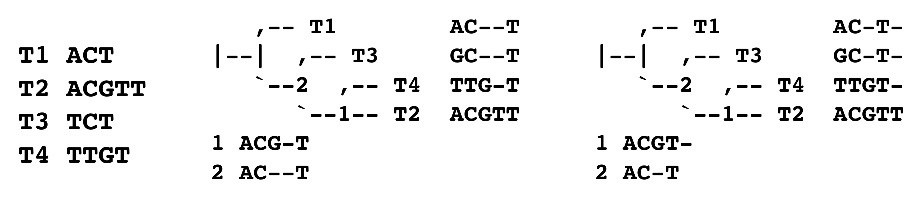
\includegraphics[scale=0.9]{figures/tut9/tap.eps}}
	{\caption[Exemplo de \textit{Tree Alignment}]{Exemplo de \textit{Tree Alignment}. Considere as sequências à esquerda. Há uma única topologia para estas sequências com o custo de 5 transformações. No entanto há dois alinhamentos implícitos relacionados a esta topologia. Para cada um deles, a atribuição dos estados nos nós é diferente.}\label{tut9:fig:tap}}
  \end{figure}

%%%%%%%%%%%%%%%%%%%%%%%%%%% FIM DA FIGURA TAP %%%%%%%%%%%%%%%%%%%%%

Análises filogenéticas de dados moleculares apresentam alguns desafios além daqueles inerentes da complexidade associada ao exame ou exploração do espaço de topologias que é uma função determinada pelo número de terminais -- como vimos no Tutorial \ref{tut3}. Dados moleculares podem variar não somente em números de elementos, isto é, estados de caracteres, mas também em tamanho (veja Tutorial \ref{tut8}). Nestes casos, tradicionalmente é feito um alinhamento a partir do qual se procede com as análises de inferência filogenética. Este alinhamento estabelece as correlações entre estados de caráter em cada coluna, considerados como proposições de homologia entre os pares de base de cada sequência dentro do contexto de homologia estática. Como visto anteriormente (seção \ref{tut8:guide_tree:trees} do Tutorial \ref{tut8}), esquemas putativos de homologia (alinhamentos) variam entre diferentes topologias utilizadas durante o alinhamento. Também foi observado que estes cenários putativos de alinhamento geram topologias com custos distintos. O conceito de homologia dinâmica \parencite[senso ][]{Wheeler_2001} integra alinhamento e busca de topologias em um único procedimento analítico conhecido como otimização direta \parencite[\textit{direct optimization};][]{Wheeler_1996}. Ao integrar esses processos analíticos, conjugamos dois níveis de complexidades, um associado ao número de topologia e o outro associado ao número de alinhamentos possíveis. 

Neste tutorial iremos explorar alguns conceitos práticos e teóricos associados à otimização direta de sequências nucleotídicas implementadas em POY \parencite[][]{VaronETAL_2010, VaronETAL_2014}. De nenhuma maneira este tutorial irá explorar toda a funcionalidade de POY e o interessado deve explorar os tutoriais disponíveis na documentação do programa (veja materiais associados a esse tutorial e literatura referenciada no final deste tutorial).

\section{Introdução ao POY}\label{tut9:context}

\subsection{Etapas de execução em POY}\label{tut9:context:steps}

O POY é um programa extremamente versátil. Parte desta versatilidade está na possibilidade de analisar simultaneamente diferentes fontes de dados (\textit{i.e.}, sequências nucleotídicas, matrizes morfológicas, entre outras), mas também na forma de interpretação e execução de \textit{scripts}. Este último componente pode ser a parte mais complexa do uso de POY e o aluno interessado em possuir melhor domínio da linguagem de \textit{script} de POY deve consultar a Seção 3.1 da documentação do programa (\texttt{tutorial\_9/literature/poy\_commands.pdf}). A execução mais simples de POY requer alguns componentes primários. O primeiro deles é a leitura dos arquivos de dados. O segundo, é a implementação da função de custo, ou seja, os parâmetros de alinhamento. Essa etapa é opcional caso o usuário queira utilizar os valores de \textit{default} do programa -- custo 1 para todas as transformações. Uma vez cumprida estas etapas, o usuário inicia a busca, seleciona a topologia mais curta e reporta o resultado. Vamos ver como isso é feito na prática.

	Em um terminal, execute:

\shellcmd{poy5s}

Você deverá obter:


\scriptsize

alan@turing:{~}\$~poy4s


Information~:~Welcome~to~POY~5.1.1~(5.1.1)

Compiled~on~Tue~Feb~23~18:59:37~BRT~2016~with~parallel~off,~interface~flat,

likelihood~on,~and~concorde~off.

Copyright~(C)~2011,~2012,~2013,~2014~Andres~Varon,~Nicholas~Lucaroni,~Lin

Hong,~Ward~Wheeler,~and~the~American~Museum~of~Natural~History.

POY~5.1.1~comes~with~ABSOLUTELY~NO~WARRANTY;~This~is~free~software,~and~you

are~welcome~to~redistribute~it~under~the~GNU~General~Public~License~Version

2,~June~1991.

\vspace{20pt}

Information~:~Setting~random~seed~value~to~1431363032

Information~:~

Information~:~

Information~:~

Information~:~For~help,~type~help().

~~~~~~~~~~~~~~

~~~~~~~~~~~~~~Enjoy!

Information~:~

~~~~~~~~~~~~~~~~Trees:

~~~~~~~~~~~~~~~~~~Storing~0~trees~

~~~~~~~~~~~~~~~~Cost~Mode:~Normal~Direct~Optimization

poy>

\normalsize
\vspace{10pt}
Nosso primeiro passo é fazer a leitura do arquivo se dados. Nesse exemplo iremos usar o arquivo \texttt{seqdata1.fas}. No \textit{prompt} de POY execute:\\

\poyprompt{read(''seqdata1.fas'')}\\

você deverá obter:\\

\scriptsize

poy>~read("seqdata1.fas")

Information~:~Reading~file~seqdata1.fas~of~type~input~sequences

Information~:

The~file~seqdata1.fas~contains~sequences~of~10~taxa,~each~sequence~holding~1

fragment.

Status~:~Loading~Trees~Finished

Information~:~
~~~~~~~~~~~~~~~~Trees:

~~~~~~~~~~~~~~~~~~Storing~0~trees~

~~~~~~~~~~~~~~~~Cost~Mode:~Normal~Direct~Optimization

poy>~
\vspace{10pt}
\normalsize

Neste exemplo, POY informa que leu o arquivo \texttt{seqdata1.fas} e que o mesmo possui um único fragmento.

Nosso próximo passo é implementar a busca; pois iremos usar as funções de custo internas do programa. Iremos fazer isso utilizando os métodos convencionais para explorar o espaço de topologias como fizemos inicialmente em TNT (\textit{i.e.}, \textbf{RAS}+\textbf{SWAP}), veja seção \ref{tut4:search} do Tutorial \ref{tut4}). Para implementar este tipo de busca são necessários dois comandos. O primeiro é o comando \texttt{build()}, que constrói árvores de Wagner à medida em que calcula o custo utilizando o algoritmo de Needleman-Wunsch \parencite{Needleman_and_Wunsch_1970}. O segundo é o comando \texttt{swap()} que executa o refinamento por SPR e TBR e, para cada rearranjo, calcula o custo da topologia da mesma forma que o fez na construção da árvore de Wagner. Vejamos isso na prática. No prompt de POY, execute:\\

\poyprompt{build(100)}\\

Observe que o comando \texttt{build()} requer um argumento que, neste caso, foi um valor numérico que é interpretado pelo POY como o número de RAS (\textit{random addition sequence} que deverá ser executado. Após a execução deste comando, você deverá obter:\\

\scriptsize

poy>~build(100)

Status~:~Wagner~:~2~of~10~--~Wagner~tree~with~cost~18.

Status~:~Wagner~:~3~of~10~--~Wagner~tree~with~cost~34.

Status~:~Wagner~:~4~of~10~--~Wagner~tree~with~cost~59.

Status~:~Wagner~:~5~of~10~--~Wagner~tree~with~cost~75.

Status~:~Wagner~:~6~of~10~--~Wagner~tree~with~cost~104.

Status~:~Wagner~:~7~of~10~--~Wagner~tree~with~cost~114.

Status~:~Wagner~:~8~of~10~--~Wagner~tree~with~cost~138.

Status~:~Wagner~:~9~of~10~--~Wagner~tree~with~cost~152.

Status~:~Wagner~Finished

Status~:~Building~Wagner~Tree~Finished

Status~:~Running~Pipeline~:~1~of~100~--~Estimated~finish~in~3~s

Status~:~Wagner~:~2~of~10~--~Wagner~tree~with~cost~24.

Status~:~Wagner~:~3~of~10~--~Wagner~tree~with~cost~39.

Status~:~Wagner~:~4~of~10~--~Wagner~tree~with~cost~64.

Status~:~Wagner~:~5~of~10~--~Wagner~tree~with~cost~88.

Status~:~Wagner~:~6~of~10~--~Wagner~tree~with~cost~101.

Status~:~Wagner~:~7~of~10~--~Wagner~tree~with~cost~112.

Status~:~Wagner~:~8~of~10~--~Wagner~tree~with~cost~129.

Status~:~Wagner~:~9~of~10~--~Wagner~tree~with~cost~155.

Status~:~Wagner~Finished

Status~:~Building~Wagner~Tree~Finished

Status~:~Running~Pipeline~:~2~of~100~--~Estimated~finish~in~2~s

...

Status~:~Wagner~Finished

Status~:~Wagner~build~:~100~of~100~--~Estimated~finish~in~0~s

Status~:~Wagner~:~2~of~10~--~Wagner~tree~with~cost~33.

Status~:~Wagner~:~3~of~10~--~Wagner~tree~with~cost~56.

Status~:~Wagner~:~4~of~10~--~Wagner~tree~with~cost~72.

Status~:~Wagner~:~5~of~10~--~Wagner~tree~with~cost~93.

Status~:~Wagner~:~6~of~10~--~Wagner~tree~with~cost~113.

Status~:~Wagner~:~7~of~10~--~Wagner~tree~with~cost~129.

Status~:~Wagner~:~8~of~10~--~Wagner~tree~with~cost~138.

Status~:~Wagner~:~9~of~10~--~Wagner~tree~with~cost~148.

Status~:~Wagner~Finished

Status~:~Wagner~build~:~101~of~100~--~Estimated~finish~in~0~s

Status~:~Wagner~build~Finished

Information~:~

~~~~~~~~~~~~~~~~Trees:

~~~~~~~~~~~~~~~~~~Storing~100~trees~with~costs~153.~to~165.

~~~~~~~~~~~~~~~~~~Best~cost~in~9~trees~

~~~~~~~~~~~~~~~~Cost~Mode:~Normal~Direct~Optimization

poy>~

\normalsize


Os resultados acima indicam que o POY contruiu 100 árvores de Wagner cujos custos variam de 153 a 165\footnote{ Estes números podem variar de execução a execução dado a aleatoriedade associada ao algoritmo.}. Dentro destas 9 delas possuem o menor custo.

Nossa próxima etapa será o refinamento destas topologias implementando rearranjos via SPR e TBR. O comando do POY para essas estratégias de refinamento é o \texttt{swap()}. Esse comando implementará os algoritmos de refinamento para todas as topologias contidas na memória. A forma mais simples de execução desse comando é a seguinte:\\

\poyprompt{swap()}\\

cujo resultado seria:\\

\scriptsize

poy>~swap()

Status~:~Tree~search~:~1~of~100~-{}-

Status~:~TBR~:~174~Searching

Status~:~TBR~Finished

...

Status~:~SPR~:~157~157.

Status~:~SPR~:~155~155.

Status~:~SPR~:~154~154.

Status~:~SPR~Finished

Status~:~Alternate~:~0~Performing~TBR~swapping

Status~:~Single~TBR~Finished

Status~:~Alternate~Finished

Status~:~Tree~search~:~100~of~100~--~Estimated~finish~in~0~s

Status~:~Alternate~:~0~Beginning~search

Status~:~Alternate~:~0~SPR~search

Status~:~SPR~:~153~153.

Status~:~SPR~Finished

Status~:~Alternate~:~0~Performing~TBR~swapping

Status~:~Single~TBR~Finished

Status~:~Alternate~Finished

Status~:~Tree~search~Finished

Information~:~

~~~~~~~~~~~~~~~~Trees:

~~~~~~~~~~~~~~~~~~Storing~100~trees~with~costs~153.~to~160.

~~~~~~~~~~~~~~~~~~Best~cost~in~38~trees~

~~~~~~~~~~~~~~~~Cost~Mode:~Normal~Direct~Optimization

poy>~

\normalsize

Após o refinamento, POY manteve 100 topologias que variaram de 153 a 160 em custo dentre as quais 38 possuem o menor custo.

Como dentro do conjunto de topologias mantidas na memória de POY há árvores subótimas, nosso próximo passo é selecionar aquelas que nos interessam. Para a seleção de topologias \textbf{únicas} e \textbf{ótimas}, utilizamos os parâmetros de \textit{default} do comando \texttt{select()}. No terminal do POY execute:\\

\poyprompt{select()}\\

você deverá obter:\\

\scriptsize

poy>~select()

Information~:~

~~~~~~~~~~~~~~~~Trees:

~~~~~~~~~~~~~~~~~~Storing~3~trees~with~costs~153.~to~153.

~~~~~~~~~~~~~~~~~~Best~cost~in~3~trees~

~~~~~~~~~~~~~~~~Cost~Mode:~Normal~Direct~Optimizationn

poy>~

\normalsize

O resultado de POY indica que foram encontradas 3 topologias com o custo de 153. Observe que antes de selecionarmos as topologias \textbf{únicas} e \textbf{ótimas} do conjunto de topologias que compilamos após o refinamento -- na etapa anterior --, haviam 38 árvores com o custo de 153. O resultado após implementarmos o comando \texttt{select()} significa que dentro deste conjunto de 38 topologias, apenas três delas eram diferentes uma das outras.

Finalmente, vamos verificar nossos resultados, ou seja, as topologias obtidas. POY imprime os resultados ou informações sobre os arquivos de entrada pelo comando \texttt{report()}. Há várias formas de obter as topologias encontradas por POY, vejamos algumas delas. No prompt de POY, execute:\\

\poyprompt{report(asciitrees)}\\

Você deverá obter as topologias encontradas impressa no terminal no formato visual com caracteres \href{http://en.wikipedia.org/wiki/ASCII}{ASCII}. Se você executar:\\

\poyprompt{report(trees:(total))}\\

Você deverá obter as topologias encontradas impressa no terminal em formato parentético (\textit{i.e., newick format}) e seus respectivos custos entre colchetes.

Finalmente, o comando \texttt{report()} permite que você direcione os resultados para arquivos e que você faça isso utilizando um ou mais arguentos. Por exemplo, se você executar:\\


\poyprompt{report("newicktrees.tre",trees,"asciitrees.txt",asciitrees)}\\

Você deverá obter dois arquivos em seu diretório de trabalho. O primeiro é o arquivo \texttt{newicktrees.tre} que conterá as topologias selecionadas em formato parentético. O segundo é o arquivo texto \texttt{asciitrees.txt} que conterá as topologias selecionadas em formato \href{http://en.wikipedia.org/wiki/ASCII}{ASCII}.

Finalmente, para sair de POY você deve digitar \texttt{exit()}.

\subsection{\textit{Scripts} de execução em POY}\label{tut9:context:scripts}

A maneira mais efetiva de utilizar o POY é utilizando \textit{scripts}. Os \textit{scripts} de POY são arquivos textos contendo os comandos de execução seguindo a estrutura analítica que acabamos de fazer. Vamos repetir o que acabamos de fazer utilizando essa forma de execução.\\

\stepcounter{ex}
\begin{blackBlock}{\textbf{Exercicio 9.\arabic{ex}}}\label{tut9:ex:9.1}

Neste exercício você deverá executar o POY utilizando um \textit{script}.

\end{blackBlock}

\begin {myindentpar}{0.3cm}
\begin{enumerate}[\itshape i.]

	\item{Crie um arquivo texto chamado \texttt{meu\_script1.poy} com o seguinte conteúdo:}

\begin{lstlisting}[caption= conteúdo do arquivo meu\_script1.poy,label=tut9:context:script1]
read("seqdata1.fas")
set(root:"Taxon1")
build(100)
swap()
select()
report("seqdata1_do.tre", trees:(total))
exit()
\end{lstlisting}

Dentre estes comandos, o único que não foi utilizado anteriormente é o comando \texttt{set(root:''Taxon1'')} -- linha 2, que indica ao POY que todas as topologias deverão ser enraizadas pelo terminal \texttt{Taxon1}.

	\item{Execute o \textit{script} \texttt{meu\_script1.poy} utilizandoo seguinte comando em seu terminal:}

\shellcmd{poy5s meu\_script1.poy}\\

Primeiro observe as últimas 31 linhas do registro de execução de POY. Você deve ter obtido:

\scriptsize

...
Status~:~Running~Pipeline~:~99~of~100~--~Estimated~finish~in~0~s

Status~:~Wagner~:~2~of~10~--~Wagner~tree~with~cost~30.

Status~:~Wagner~:~3~of~10~--~Wagner~tree~with~cost~54.

Status~:~Wagner~:~4~of~10~--~Wagner~tree~with~cost~66.

Status~:~Wagner~:~5~of~10~--~Wagner~tree~with~cost~87.

Status~:~Wagner~:~6~of~10~--~Wagner~tree~with~cost~113.

Status~:~Wagner~:~7~of~10~--~Wagner~tree~with~cost~118.

Status~:~Wagner~:~8~of~10~--~Wagner~tree~with~cost~139.

Status~:~Wagner~:~9~of~10~--~Wagner~tree~with~cost~146.

Status~:~Wagner~Finished

Status~:~Building~Wagner~Tree~Finished

Status~:~Alternate~:~0~Beginning~search

Status~:~Alternate~:~0~SPR~search

Status~:~SPR~:~158~158.

Status~:~SPR~:~156~156.

Status~:~SPR~Finished

Status~:~Alternate~:~0~Performing~TBR~swapping

Status~:~Single~TBR~Finished

Status~:~Alternate~Finished

Status~:~Running~Pipeline~:~100~of~100~--~Estimated~finish~in~0~s

Status~:~Running~Pipeline~Finished

Status~:~Diagnosis~:~0~Recalculating~original~tree

Status~:~Diagnosis~Finished

Status~:~Diagnosis~:~1~of~3~--~Recalculating~trees

Status~:~Diagnosis~:~0~Recalculating~original~tree

Status~:~Diagnosis~Finished

Status~:~Diagnosis~:~2~of~3~--~Recalculating~trees

Status~:~Diagnosis~:~0~Recalculating~original~tree

Status~:~Diagnosis~Finished

Status~:~Diagnosis~:~3~of~3~--~Recalculating~trees

Status~:~Diagnosis~Finished

\normalsize

Quando POY executa um \textit{script}, as instruções de execução funcionam de uma forma um pouco diferente em comparação com os comandos que você executou passo a passo anteriormente. No exemplo da seção \ref{tut9:context:steps}, POY construiu todas as \textbf{RAS} para depois fazer o refinamento via SPR+TBR. Quando executado via \textit{script}, POY faz o refinamento logo após a construção da árvore de Wagner e retém a(s) topologia(s) de menor custo. O resultado da análise pode ser verificado no arquivo \texttt{seqdata1\_do.tre} que contém 3 topologias com o custo de 153:\\

\scriptsize

\texttt{(Taxon1,((Taxon4,(Taxon3,Taxon5)),((Taxon7,Taxon8),(Taxon9,(Taxon10,(Taxon2,Taxon6))))));}\\
\texttt{(Taxon1,((Taxon4,(Taxon3,Taxon5)),(Taxon10,((Taxon2,Taxon6),(Taxon9,(Taxon7,Taxon8))))));}\\
\texttt{(Taxon1,((Taxon4,(Taxon3,Taxon5)),((Taxon9,(Taxon2,Taxon6)),(Taxon10,(Taxon7,Taxon8)))));}\\

\normalsize

Finalmente, vale ressaltar que a versão mais rescente de POY (atualmente 5.1.1) atribui custos idênticos para qualquer tipo de transformação (\textit{i.e.}, substituições e INDELs) ao passo que nas versões anteriores a razão de custos entre INDELs:substituições é de 2:1.


	\item{Os dados utilizados neste exercício são os mesmos que você utilizou no Tutorial \ref{tut8} na seção \ref{tut8:msa}. Compare os resultados de POY com aqueles obtidos por homologia estática registrados nas Tabelas \ref{tut8:table:align} e \ref{tut8:table:align} do Tutorial \ref{tut8} e responda:}

	\begin {myindentpar}{0.5cm}
	\begin{enumerate}[\itshape a.]

	\item{O custo obtido em POY é melhor ou pior do que os resultados que você havia obtido?}\\
		\line(1,0){400}\\
		\line(1,0){400}\\

	\item{As topologias diferem?}\\
		\line(1,0){400}\\
		\line(1,0){400}\\

	\end{enumerate}
	\end{myindentpar}

\end{enumerate}
\end{myindentpar}


\subsection{Análises simultâneas em POY}\label{tut9:context:partitions}

Um dos componentes mais interessantes de POY é a possibilidade de analisar diferentes fontes de dados simultaneamente. Considere que você possui 3 partições com propriedades analíticas distintas. Suponha que você tenha uma partição que está sujeita a alinhamento, pois as sequências diferem de tamanho, uma outra partição cujos dados genotípicos provém de uma região codificadora que não contém INDELs, e ainda uma matriz de dados fenotípicos. Dentro do conceito de homologia estática, o procedimento analítico a ser adotado seria o alinhamento da primeira partição que posteriormente seria concatenada com as demais partições e este conjunto de dados seria submetido à análise filogenética. No entanto, considere que o alinhamento da primeira partição depende de uma topologia para a qual as demais partições não possuem nenhuma influência. No exemplo que se segue iremos explorar como POY analisaria essas partições simultaneamente.

	Considere os seguintes conjuntos de dados:

\begin {myindentpar}{0.5cm}
\begin{enumerate}[\itshape 1.]

	\item{partition1.fas -- dados não sujeitos a alinhamento}
	\item{partition2.fas -- dados sujeitos a alinhamento\footnote{ Estes dados encontram-se alinhados, porém POY irá desconsiderar os \textit{gaps} a não ser que você especifique ao programa que esta partição deva ser considerada como pré-alinhada (veja abaixo)}}
	\item{partition3.tnt -- dados fenotípicos}

\end{enumerate}
\end{myindentpar}

Dentre as partições apresentadas acima, \texttt{partition1.fas} e \texttt{partition3.tnt} não devam ser submetidas á otimização direta ao passo que a \texttt{partition2.fas} deverá ser analisada por homologia dinâmica. A implementação de uma análise em POY que leve em consideração as propriedades destas partições requer a estrutura ilustrada no \texttt{script} abaixo (Script \ref{tut9:context:script2}):\\


\begin{lstlisting}[caption= conteúdo do arquivo partitions\_script.poy,label=tut9:context:script2]
read(prealigned:("partition1.fas"))
read("partition2.fas","partition3.tnt")
set(root:"Taxon1")
build(100)
swap()
select()
report(trees, treestats)
exit()
\end{lstlisting}

Este \textit{script} está contido no arquivo \texttt{partitions\_script.poy}. Na linha 1, POY lê os arquivos \texttt{partition1.fas} no qual o argumento \texttt{prealigned} do comando \texttt{read} informa ao POY que o arquivo \texttt{partition1.fas} contém sequências nucleotídicas pré-alinhadas. A linha 2, instrui o POY a ler os arquivos \texttt{partition2.fas}  e \texttt{partition3.tnt} e considera que o primeiro será submetido à otimização direta ao passo que o segundo é uma matriz de dados de homologia estática -- no caso, dados fenotípicos. Finalmente, o comando \texttt{report()} contém dois argumentos, \texttt{trees, treestats}, cujo primeiro retorna a(s) topologia(a) encontrada(s) e o segundo o custo da(s) mesma(s). Ao executá-lo você deverá obter:\\

\scriptsize

...

Status~:~Wagner~Finished

Status~:~Building~Wagner~Tree~Finished

Status~:~Alternate~:~0~Beginning~search

Status~:~Alternate~:~0~SPR~search

Status~:~SPR~:~376~376.

Status~:~SPR~:~375~375.

Status~:~SPR~Finished

Status~:~Alternate~:~0~Performing~TBR~swapping

Status~:~Single~TBR~Finished

Status~:~Alternate~Finished

Status~:~Running~Pipeline~:~100~of~100~--~Estimated~finish~in~0~s

Status~:~Running~Pipeline~Finished

Information~:~Vectorized:8~of~8~characters.

Status~:~Diagnosis~:~0~Recalculating~original~tree

Status~:~Diagnosis~Finished

Status~:~Diagnosis~:~1~of~1~--~Recalculating~trees

Status~:~Diagnosis~Finished

(Taxon1,((Taxon5,(Taxon2,(Taxon4,Taxon9))),(Taxon6,(Taxon8,(Taxon3,(Taxon10,Taxon7))))))

;

\vspace{20pt}

Trees~Found:

~~~~~~~~~~~~~~~~~~~~~~~~~~~~~~~~~~~~~~~~~~~~

Tree~length~~~~Number~of~hits

370.~~~~~~~~~~~1

\normalsize

	A análise destas partições resulta em uma única topologia com o custo de 370.\\

\vspace{30pt}

\stepcounter{ex}
\begin{blackBlock}{\textbf{Exercicio 9.\arabic{ex}}}\label{tut9:ex:9.2}

Neste exercício você deverá fazer uma análise de cada partição destes dados e comparar os resultados das análises individuais com a análise simultânea. Para cada análise, registre as topologias no espaço abaixo e responda:

\end{blackBlock}


\newpage
Topologias encontradas nas análises filogenéticas das partições do Exercício 9.2:

\begin{center}
\fbox{\parbox[c][10cm][s]{6.5cm}{\texttt{Análise simultânea}}}
\fbox{\parbox[c][10cm][s]{6.5cm}{\texttt{Partição 1}}}\\
\fbox{\parbox[c][10cm][s]{6.5cm}{\texttt{Partição 2}}}
\fbox{\parbox[c][10cm][s]{6.5cm}{\texttt{Partição 3}}}\\
\end{center}

\vspace{5pt}

\begin {myindentpar}{0.3cm}
\begin{enumerate}[\itshape i.]

	\item{As topologias são idênticas?}

\line(1,0){400}\\
\line(1,0){400}\\


	\item{Para cada clado presente na análise simultânea, identique se eles são corroborados pelas partições. Você considera que alguma partição tem maior influência na estrutura cladistica (topologia) recuperada na análise simultânea?}

\line(1,0){400}\\
\line(1,0){400}\\

	\item{Considerando o número de caracteres de cada partição, existe alguma relação entre número de caracteres das partições e a influência na estutura da topologia da análise simultânea?}

\line(1,0){400}\\
\line(1,0){400}\\

\end{enumerate}
\end{myindentpar}

\subsection{Implementação de matrizes de custo em POY}\label{tut9:context:tcm}

A implementação de parâmetros de alinhamento ( = função de custo) em POY é feita pelo comando ``\texttt{transform()}'' e o argumento ``\texttt{tcm:}''. Este argumento define a matriz de custo de transformação para conjuntos de caracteres. O \textit{default} de POY é \texttt{tcm:(1,1)}, no qual o custo para substituições e INDELs, respectivamente é 1. Em versões anteriores de POY, o custo de INDELs era 2, portanto, o argumento seria expresso como \texttt{tcm:(1,2)}. Para o exemplo anterior, há duas formas de implementar matrizes de custo de transformação. Na primeira delas, o Script \ref{tut9:context:script2} seria modificado da seguinte maneira:\\


\begin{lstlisting}[caption= Modificação do arquivo partitions\_script.poy para implementar matriz de custo de transformação.,label=tut9:context:script3]
read(prealigned:("partition1.fas"))
read("partition2.fas","partition3.tnt")
transform(tcm:(1,2))
set(root:"Taxon1")
build(100)
swap()
select()
report(trees, treestats)
exit()
\end{lstlisting}

Neste \textit{script} a linha 3 implementa os custos de transformação para todos os caracteres no qual o valor atribuído para substituições e INDELs é 1 e 2, respectivamente. No entanto, observe que somente uma das partições possuí INDELs e talvez seja desejável especificar para qual destas partições POY deverá considerar a matriz de custo em questão. Se modificarmos o Script \ref{tut9:context:script3} da seguinte maneira:

\begin{lstlisting}[caption= Modificação do arquivo partitions\_script.poy para implementar matriz de custo de transformação para a partição \texttt{partition2.fas}.,label=tut9:context:script4]
read(prealigned:("partition1.fas"))
read("partition2.fas","partition3.tnt")
transform(names:("partition2.fas"),(tcm:(1,2)))
set(root:"Taxon1")
build(100)
swap()
select()
report(trees, treestats)
exit()
\end{lstlisting}

Neste caso, o argumento ``\texttt{names:}'' identifica a partição \texttt{partition2.fas} para qual a matriz de custo de transformação ``\texttt{tcm:(1,2)}'' será implementada.

Outra forma de implementar matrizes de custo em POY é utilizando arquivos que contém os custos de transformação. Estas matrizes são matrizes 5x5, no caso de sequências nucleotídicas, nas quais são especificadas os custos de transformação para cada estado (\textit{i.e.}, \texttt{INDELs}, \texttt{A}, \texttt{C}, \texttt{G} e \texttt{T}). Por exemplo, verifique o conteúdo do arquivo 2111.tcm:

\texttt{0 1 1 1 2}

\texttt{1 0 1 1 2}

\texttt{1 1 0 1 2}

\texttt{1 1 1 0 2}

\texttt{2 2 2 2 0}\\

	Esta matriz especifica as seguintes transformações:


\texttt{~~~[A][C][G][T][-]}

\texttt{[A]~0~~1~~1~~1~~2}

\texttt{[C]~1~~0~~1~~1~~2}

\texttt{[G]~1~~1~~0~~1~~2}

\texttt{[T]~1~~1~~1~~0~~2}

\texttt{[-]~2~~2~~2~~2~~0}\\

Essa é uma forma mais versátil de implementar matrizes de custo, pois possibilita que o usuário atribua custos diferenciais para determinados tipos de transformação (\textit{e.g.}, transições e transversões). A linha de comando que implementa matrizes de custo expressas em arquivos com esse conteúdo é ilustrado na modificação do Script \ref{tut9:context:script4} feita abaixo:\\

\begin{lstlisting}[caption= Modificação do arquivo partitions\_script.poy para implementar matriz de custo de transformação para a partição \texttt{partition2.fas}.,label=tut9:context:script4]
read(prealigned:("partition1.fas"))
read("partition2.fas","partition3.tnt")
transform(names:("partition2.fas"),(tcm:("211.tcm")))
set(root:"Taxon1")
build(100)
swap()
select()
report(trees, treestats)
exit()
\end{lstlisting}

\vspace{10pt}

\stepcounter{ex}
\begin{blackBlock}{\textbf{Exercicio 9.\arabic{ex}}}\label{tut9:ex:9.3}

Neste exercício você deverá executar 2 análises em POY para os dados contidos nos arquivos \texttt{partition1.fas}, \texttt{partition2.fas} e \texttt{partition3.tnt} em que o custo para INDELs seja 2 e 4. As topologias resultantes destas análises deverão ilustradas no espaço abaixo e você deverá comentar se os resultados diferem da análise anterios na qual os custos para INDELs e substituições eram idênticos.

\end{blackBlock}

\begin{center}
\fbox{\parbox[c][7.5cm][s]{5.5cm}{\texttt{tcm:(1,2)}}}
\fbox{\parbox[c][7.5cm][s]{5.5cm}{\texttt{tcm:(1,4)}}}\\
\vspace{30pt}
\line(1,0){400}\\
\line(1,0){400}\\
\line(1,0){400}\\
\end{center}



%%%%%%%%%%%%%%%%%%%%%%%%%%%% HERE ENDS TEXT AND ADDS REFERENCES %%%%%%%%%%%%%%%%%%%%%%%%%%%% 
\section{Referências}\label{tut9:refs}
\printbibliography[heading=none]
\end{refsection}
%  
